% !TeX encoding = UTF-8
% !TeX program = xelatex
% !TeX spellcheck = en_US

\documentclass[a4paper]{ltxdoc}
\usepackage{amsmath}
\usepackage[UTF8]{ctex}
\usepackage{unicode-math}
\usepackage{caption}
\usepackage{booktabs}
\usepackage{xcolor}
\usepackage{array}
\usepackage{listings}
\usepackage[perpage]{footmisc}
\usepackage{hypdoc}
\usepackage{geometry}
\usepackage{endnotes}
\usepackage{graphicx}
\usepackage{multirow}
\usepackage{longtable}
% \usepackage[multiple]{endnotes}
\usepackage{multicol}
\usepackage{blindtext}
\geometry{a4paper, scale=0.85}
\newenvironment{Figure}
  {\par\medskip\noindent\minipage{\linewidth}}
  {\endminipage\par\medskip}


\title {实验报告\\光电效应测量普朗克常数}
\author {少年班学院\\马天开 PB21000030(2号)}
\date {\today}


\begin{document}
\begin{multicols}{2}
    \maketitle
    \section{实验原理}
    单色光照射在光电管的阴极上有电子发射出来的现象叫光电效应,出射的电子称之为光电子,形成的电流称之为光电流。光电流很弱。加载在光电管中阳极与阴极之间电压为正值时,随着电压的增大光电流迅速增大,电压增大到一定值后,光电流趋于饱和。加载在阳极与阴极之间电压为负值时,随着电压数值逐渐变大,光电流变弱,负电压数值增大到 $U_0$ 值时,光电流变为零。把电压 $U_0$ 称之为遏止电压。本实验要求测量 5 种不同单色光分别照射下,光电流的遏止电压值。本实验还需测量和验证饱和光电流与光强之间的关系,是否满足线性正比关系。

    补充内容:测量 5 种不同单色光分别照射下,光电管完整的伏安特性曲线,以及基于此曲线分析和测量出光电流的遏止电压(拐点法)。

    \section{零电流法、补偿法测量遏止电压}
    \begin{itemize}
        \item 实验内容:

              固定一种直径大小的光阑的情况下,分别测量5种不同单色光的照射下,光电流的遏止电压。

        \item 实验原理:
              根据:
              $$
                  \left\{
                  \begin{aligned}
                      h \upsilon & = \dfrac 1 2 m v_{0}^2 + A \\
                      eU_0       & = \dfrac 1 2 m v_0^2       \\
                  \end{aligned}
                  \right.
              $$
              得到:
              \begin{equation}
                  eU_0 = h\upsilon - A
              \end{equation}
        \item 实验数据:


              (本文中默认单位:$\lambda: nm,\Phi: mm,I: 10^{-10} A$)
              \bigskip
              \begin{Figure}
                  \centering
                  $\Phi = 4 mm$

                  \smallskip
                  \begin{tabular}{|c|c|c|c|}
                      \hline $\lambda _i$ & $v$   & $U_{0i}$ & $U_{0i} \prime$ \\
                      \hline 365.0        & 8.214 & 1.724    & 1.730           \\
                      \hline 404.7        & 7.408 & 1.496    & 1.502           \\
                      \hline 435.8        & 6.879 & 1.178    & 1.180           \\
                      \hline 546.1        & 5.480 & 0.612    & 0.614           \\
                      \hline 577.0        & 5.196 & 0.494    & 0.498           \\ \hline
                  \end{tabular}
              \end{Figure}

        \item 数据处理

              对$U_0 - \upsilon,U_0\prime - \upsilon$ 进行线性回归分析:

              \begin{Figure}
                  \centering
                  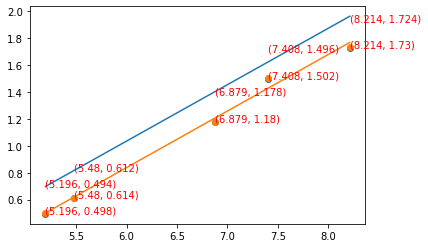
\includegraphics[width=\linewidth]{img/5.png}
              \end{Figure}

              线性回归的结果:
              $$
                  \left\{
                  \begin{aligned}
                      U_0       & = 0.41893012 \cdot \upsilon - 1.67896893  \\
                      U_0\prime & =  0.41992569 \cdot \upsilon - 1.68157493
                  \end{aligned}
                  \right.
              $$

              利用补偿法测出的结果,得到:
              $$
                  h= k \cdot e \approx 6.728 \times 10^{-34} J\cdot s
              $$

              与公认值$h_0 = 6.626 \times 10^{-34} J\cdot s$的相对误差:

              $$\Delta = 1.539\%$$

              令上面$U_0 =0$,解出:$\upsilon _0 = 4.088 \times 10^{14} s^{-1}$,对应$\lambda_0 = 748.5 nm$,此即波长红限。

              逸出功:$A=e\cdot b=2.68\times 10^{-19} J$
    \end{itemize}
    \section{测量饱和光电流与光强的关系}
    \subsection{测量光阑孔径与光电流的关系}
    \begin{itemize}
        \item 实验内容:

              选择一种单色光,固定光电管阴阳极电压(在饱和区),改变不同的光阑(直径$\Phi$)大小,来改变光强。

        \item 实验数据:

              \smallskip
              \begin{Figure}
                  \centering
                  $\lambda = 435.8 mm,U_{AK} = 40 V, l =400mm$

                  \smallskip
                  \begin{tabular}{|c|c|}
                      \hline $\Phi$ & $I_1$ \\
                      \hline 14.35  & 406.0 \\
                      \hline 8      & 117.2 \\
                      \hline 4      & 28.0  \\
                      \hline 2      & 8.2   \\
                      \hline
                  \end{tabular}
              \end{Figure}
              \begin{Figure}
                  \centering
                  $\lambda = 546.1 mm,U_{AK} = 40 V, l =400mm$

                  \smallskip
                  \begin{tabular}{|c|c|}
                      \hline $\Phi$ & $I_2$ \\
                      \hline 14.35  & 31.1  \\
                      \hline 8      & 8.2   \\
                      \hline 4      & 1.8   \\
                      \hline 2      & 0.5   \\
                      \hline
                  \end{tabular}
              \end{Figure}
        \item 数据分析:

              %   显然,发光强度$l \propto \Phi ^2$,假定光电流与光强之间满足$I \propto l^k$

              对于$\ln I_1 - \ln \Phi,\ln I_2 - \ln \Phi$进行回归分析,得到:
              \begin{Figure}
                  \centering
                  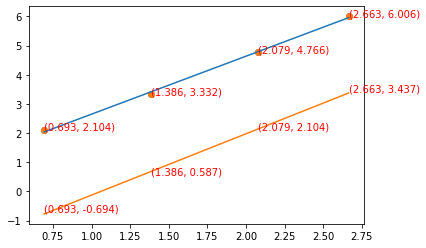
\includegraphics[width=\linewidth]{img/3.png}
              \end{Figure}
              % Not finished
              回归的结果:
              $$
                  \left\{
                  \begin{aligned}
                      \ln I_1 & = 1.987 \ln \Phi +0.663 \\
                      \ln I_2 & = 2.102 \ln \Phi -2.227
                  \end{aligned}
                  \right.
              $$

              发光强度与直径之间满足:$l \propto \Phi ^2$,因此光电流$I \propto \Phi ^{1.987} \approx \Phi ^2 \propto l$
    \end{itemize}
    \subsection{测量光源距离和光电流的关系}
    \begin{itemize}
        \item 实验内容:

              选择一种单色光,固定光电管阴阳极电压(在饱和区),改变光电管与汞灯光源的距离($l$),来改变光强。

        \item 实验数据:

              \smallskip
              \begin{Figure}
                  \centering
                  $\lambda = 435.8 mm,U_{AK} = 50 V, \Phi = 4mm$

                  \smallskip
                  \begin{tabular}{|c|c|}
                      \hline $L$ & $I$  \\
                      \hline 400 & 29.2 \\
                      \hline 380 & 34.1 \\
                      \hline 360 & 39.4 \\
                      \hline 340 & 46.9 \\
                      \hline 320 & 56.0 \\
                      \hline 300 & 67.5 \\
                      \hline
                  \end{tabular}
              \end{Figure}
              \begin{Figure}
                  \centering
                  $\lambda = 546.1 mm,U_{AK} = 50 V, \Phi = 4mm$

                  \smallskip
                  \begin{tabular}{|c|c|}
                      \hline $L$ & $I$  \\
                      \hline 400 & 19.2 \\
                      \hline 380 & 22.4 \\
                      \hline 360 & 26.1 \\
                      \hline 340 & 31.7 \\
                      \hline 320 & 38.4 \\
                      \hline 300 & 45.8 \\
                      \hline
                  \end{tabular}
              \end{Figure}
        \item 数据分析:

              对于$\ln I_1 - \ln L,\ln I_2 - \ln L$进行回归分析,得到:
              \begin{Figure}
                  \centering
                  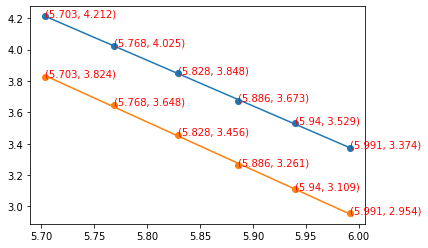
\includegraphics[width=\linewidth]{img/6.png}
              \end{Figure}
              回归的结果:
              $$
                  \left\{
                  \begin{aligned}
                      \ln I_1 & = -2.910 \ln L + 20.812 \\
                      \ln I_2 & = -3.062 \ln L + 21.296
                  \end{aligned}
                  \right.
              $$

              发光强度与到光源的距离满足:$l \propto L^{-3}$,因此光电流$I \propto L^{-2.986} \approx L^{-3} \propto l$
    \end{itemize}
    \section{“拐点法”测量光电流的遏止电压}
    \begin{itemize}
        \item 实验内容:

              测量完整的伏安特性曲线,以及使用“拐点法”测量光电流的遏制电压。计算普朗克常数$h$。

        \item 实验数据:

              实验数据放在文章末尾。

        \item 数据分析:

              首先对$I-U$作图,得到:
              \begin{Figure}
                  \centering
                  $\Phi = 4mm, -2V\leq U\leq 50V$
                  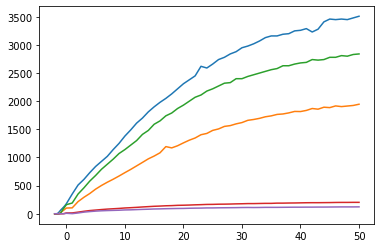
\includegraphics[width=\linewidth]{img/7.png}
              \end{Figure}

              可以看到当$U_0$较小时,图像存在较为明显的拐点:
              \begin{Figure}
                  \centering
                  $\Phi = 4mm, -2V\leq U\leq 0V$
                  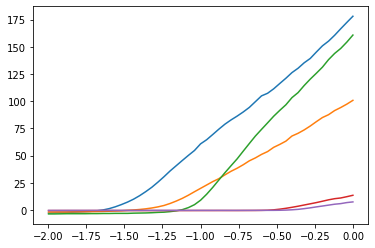
\includegraphics[width=\linewidth]{img/8.png}
              \end{Figure}

              以$365 mm$单色光为例
              在$-2V \sim 0 V$之间拟合的结果为:
              \begin{Figure}
                  \centering
                  $\Phi = 4mm, \lambda = 365mm, -2V\leq U\leq 0V$
                  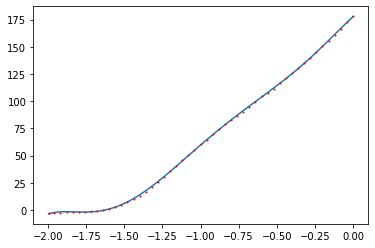
\includegraphics[width=\linewidth]{img/10.png}
              \end{Figure}

              对拟合的结果取二阶偏导;得到拐点:$x_0=-1.87V$;根据拐点法的要求,对$x \in (-2,x_0)$中的点进行线性回归,绘制得到:
              \begin{Figure}
                  \centering
                  $\Phi = 4mm, \lambda = 365mm, -2V\leq U\leq 0V$
                  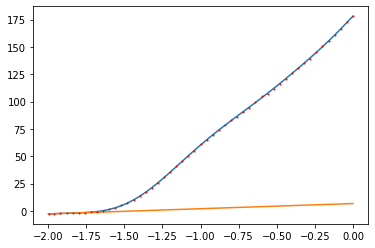
\includegraphics[width=\linewidth]{img/11.png}
              \end{Figure}

              将数据进行补偿后,测算截止电压$U_0 = 1.70V$。

              \bigskip
              用相同的办法处理余下数据,可以得到下表:

              \begin{Figure}
                  \centering
                  $\Phi = 4 mm$

                  \smallskip
                  \begin{tabular}{|c|c|c|}
                      \hline $\lambda _i$ & $v$   & $U_{0i}$ \\
                      \hline 365.0        & 8.214 & 1.896    \\
                      \hline 404.7        & 7.408 & 1.786    \\
                      \hline 435.8        & 6.879 & 1.447    \\
                      \hline 546.1        & 5.480 & 0.787    \\
                      \hline 577.0        & 5.196 & 0.751    \\ \hline
                  \end{tabular}
              \end{Figure}

              线性回归的结果:
              \begin{Figure}
                  \centering
                  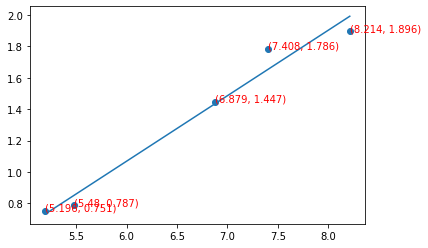
\includegraphics[width=\linewidth]{img/12.png}
              \end{Figure}

              通过与上面相同的方法,测算$h$的值为:
              $$
                  h = 6.685 \times 10^{-34} J \cdot s
              $$

              与公认值$h_0 = 6.626$的相对误差为:
              $$
                  \Delta = 0.890\%
              $$
    \end{itemize}

    \section{另附}
    \begin{itemize}
        % \item 数据分析所使用的Python 代码
        \item 拐点法实验数据
        \item 拐点法函数图像(经过拟合)
    \end{itemize}
\end{multicols}
\newpage
\section*{附1:实验数据}
% \resizebox{0.5}{!}{
\small{
    \begin{longtable}{|l|l|l|l|l|l|}
        \hline
        U/V & I/$10^{-12}A$ & I/$10^{-12}A$ & I/$10^{-12}A$ & I/$10^{-12}A$ & $I/10^{-12}A$ \\ \hline
        ~   & 365nm         & 405nm         & 436nm         & 546nm         & 577nm         \\ \hline
        -1  & 70            & 0             & 0             & 0             & 0             \\ \hline
        0   & 80            & 21            & 40            & 0             & 0             \\ \hline
        1   & 350           & 104           & 190           & 14            & 1             \\ \hline
        2   & 510           & 215           & 350           & 28            & 13            \\ \hline
        3   & 610           & 292           & 460           & 43            & 28            \\ \hline
        4   & 730           & 359           & 580           & 56            & 38            \\ \hline
        5   & 840           & 437           & 680           & 65            & 46            \\ \hline
        6   & 930           & 502           & 790           & 74            & 52            \\ \hline
        7   & 1020          & 560           & 880           & 82            & 56            \\ \hline
        8   & 1140          & 613           & 970           & 88            & 59            \\ \hline
        9   & 1250          & 670           & 1070          & 94            & 62            \\ \hline
        10  & 1380          & 730           & 1140          & 102           & 67            \\ \hline
        11  & 1490          & 788           & 1220          & 107           & 69            \\ \hline
        12  & 1610          & 850           & 1300          & 113           & 73            \\ \hline
        13  & 1700          & 912           & 1410          & 120           & 77            \\ \hline
        14  & 1810          & 975           & 1480          & 126           & 80            \\ \hline
        15  & 1900          & 1025          & 1590          & 132           & 84            \\ \hline
        16  & 1980          & 1083          & 1650          & 136           & 86            \\ \hline
        17  & 2050          & 1193          & 1740          & 141           & 89            \\ \hline
        18  & 2130          & 1170          & 1790          & 144           & 91            \\ \hline
        19  & 2220          & 1208          & 1870          & 149           & 93            \\ \hline
        20  & 2310          & 1259          & 1930          & 151           & 94            \\ \hline
        21  & 2380          & 1307          & 2000          & 154           & 97            \\ \hline
        22  & 2450          & 1346          & 2070          & 158           & 99            \\ \hline
        23  & 2620          & 1404          & 2110          & 161           & 100           \\ \hline
        24  & 2590          & 1427          & 2180          & 165           & 103           \\ \hline
        25  & 2660          & 1481          & 2220          & 166           & 103           \\ \hline
        26  & 2740          & 1507          & 2270          & 169           & 105           \\ \hline
        27  & 2780          & 1552          & 2320          & 170           & 106           \\ \hline
        28  & 2840          & 1566          & 2330          & 172           & 107           \\ \hline
        29  & 2880          & 1597          & 2400          & 175           & 108           \\ \hline
        30  & 2950          & 1620          & 2400          & 177           & 110           \\ \hline
        31  & 2980          & 1660          & 2440          & 180           & 111           \\ \hline
        32  & 3020          & 1675          & 2470          & 180           & 110           \\ \hline
        33  & 3070          & 1695          & 2500          & 182           & 111           \\ \hline
        34  & 3130          & 1723          & 2530          & 184           & 113           \\ \hline
        35  & 3160          & 1739          & 2560          & 184           & 113           \\ \hline
        36  & 3160          & 1765          & 2580          & 188           & 113           \\ \hline
        37  & 3190          & 1773          & 2630          & 188           & 114           \\ \hline
        38  & 3200          & 1792          & 2630          & 190           & 115           \\ \hline
        39  & 3250          & 1818          & 2660          & 191           & 116           \\ \hline
        40  & 3260          & 1816          & 2680          & 193           & 116           \\ \hline
        41  & 3290          & 1836          & 2690          & 195           & 117           \\ \hline
        42  & 3230          & 1870          & 2740          & 196           & 117           \\ \hline
        43  & 3280          & 1858          & 2730          & 196           & 118           \\ \hline
        44  & 3410          & 1893          & 2740          & 197           & 118           \\ \hline
        45  & 3460          & 1886          & 2780          & 198           & 119           \\ \hline
        46  & 3450          & 1916          & 2780          & 200           & 120           \\ \hline
        47  & 3460          & 1904          & 2810          & 201           & 121           \\ \hline
        48  & 3450          & 1914          & 2800          & 201           & 121           \\ \hline
        49  & 3480          & 1924          & 2830          & 202           & 121           \\ \hline
        50  & 3510          & 1946          & 2840          & 202           & 122           \\ \hline
    \end{longtable}}
% \newpage
\small{
    \begin{longtable}{|l|l|l|l|l|l|}
        \hline
        U/V    & I/$10^{-12}A$ & I/$10^{-12}A$ & I/$10^{-12}A$ & I/I/$10^{-12}A$ & I/$10^{-12}A$ \\ \hline
        ~      & 365nm         & 405nm         & 436nm         & 546nm           & 577nm         \\ \hline
        -1.998 & -2.8          & -1.88         & -3.6          & -0.54           & -0.4          \\ \hline
        -1.96  & -2.56         & -1.88         & -3.6          & -0.53           & -0.39         \\ \hline
        -1.92  & -2.4          & -1.85         & -3.5          & -0.52           & -0.39         \\ \hline
        -1.88  & -2.23         & -1.88         & -3.4          & -0.51           & -0.39         \\ \hline
        -1.84  & -2.03         & -1.76         & -3.4          & -0.53           & -0.37         \\ \hline
        -1.8   & -1.83         & -1.72         & -3.4          & -0.52           & -0.38         \\ \hline
        -1.76  & -1.58         & -1.63         & -3.4          & -0.53           & -0.38         \\ \hline
        -1.72  & -1.24         & -1.54         & -3.3          & -0.52           & -0.37         \\ \hline
        -1.68  & -0.73         & -1.45         & -3.3          & -0.51           & -0.38         \\ \hline
        -1.64  & 0.06          & -1.32         & -3.2          & -0.5            & -0.39         \\ \hline
        -1.6   & 1.26          & -1.14         & -3.2          & -0.5            & -0.39         \\ \hline
        -1.56  & 2.93          & -0.92         & -3.1          & -0.51           & -0.38         \\ \hline
        -1.52  & 4.97          & -0.72         & -3.1          & -0.51           & -0.39         \\ \hline
        -1.48  & 7.25          & -0.33         & -3.1          & -0.51           & -0.38         \\ \hline
        -1.44  & 9.94          & 0.03          & -2.9          & -0.52           & -0.37         \\ \hline
        -1.4   & 13.17         & 0.48          & -2.8          & -0.51           & -0.37         \\ \hline
        -1.36  & 16.87         & 1.08          & -2.7          & -0.5            & -0.37         \\ \hline
        -1.32  & 20.9          & 1.85          & -2.5          & -0.5            & -0.38         \\ \hline
        -1.28  & 25.6          & 2.86          & -2.2          & -0.49           & -0.38         \\ \hline
        -1.24  & 30.6          & 4.16          & -2            & -0.5            & -0.39         \\ \hline
        -1.2   & 35.9          & 6             & -1.5          & -0.51           & -0.38         \\ \hline
        -1.16  & 40.7          & 8.2           & -0.8          & -0.51           & -0.36         \\ \hline
        -1.12  & 45.5          & 10.7          & 0.3           & -0.5            & -0.36         \\ \hline
        -1.08  & 50.2          & 13.6          & 2.2           & -0.51           & -0.34         \\ \hline
        -1.04  & 54.7          & 16.8          & 4.9           & -0.49           & -0.36         \\ \hline
        -1     & 60.8          & 19.9          & 9             & -0.49           & -0.35         \\ \hline
        -0.96  & 64.6          & 23            & 14.5          & -0.48           & -0.35         \\ \hline
        -0.92  & 69.4          & 26.1          & 20.8          & -0.48           & -0.36         \\ \hline
        -0.88  & 74.3          & 28.8          & 27.6          & -0.47           & -0.36         \\ \hline
        -0.84  & 78.9          & 32.3          & 34.3          & -0.48           & -0.35         \\ \hline
        -0.8   & 82.8          & 35.6          & 40.7          & -0.48           & -0.36         \\ \hline
        -0.76  & 86.3          & 38.4          & 47            & -0.48           & -0.36         \\ \hline
        -0.72  & 90.1          & 41.6          & 54.1          & -0.46           & -0.35         \\ \hline
        -0.68  & 94.3          & 45.2          & 61.1          & -0.44           & -0.34         \\ \hline
        -0.64  & 99.6          & 47.9          & 68            & -0.42           & -0.33         \\ \hline
        -0.6   & 104.9         & 51.1          & 74.1          & -0.35           & -0.32         \\ \hline
        -0.56  & 107.3         & 53.7          & 80.1          & -0.21           & -0.32         \\ \hline
        -0.52  & 111.4         & 57.6          & 86.2          & 0.16            & -0.31         \\ \hline
        -0.48  & 116.3         & 60.3          & 91.6          & 0.77            & -0.24         \\ \hline
        -0.44  & 121.1         & 63.3          & 96.7          & 1.55            & -0.09         \\ \hline
        -0.4   & 126.3         & 68            & 103.3         & 2.48            & 0.19          \\ \hline
        -0.36  & 130.3         & 70.5          & 107.9         & 3.48            & 0.6           \\ \hline
        -0.32  & 135.3         & 73.6          & 114.4         & 4.59            & 1.24          \\ \hline
        -0.28  & 139.3         & 77.2          & 120.3         & 5.69            & 1.99          \\ \hline
        -0.24  & 145.2         & 81.2          & 125.7         & 6.81            & 2.85          \\ \hline
        -0.2   & 150.9         & 85            & 131.3         & 8.06            & 3.65          \\ \hline
        -0.16  & 155.2         & 87.6          & 138.2         & 9.35            & 4.48          \\ \hline
        -0.12  & 160.6         & 91.4          & 143.9         & 10.4            & 5.32          \\ \hline
        -0.08  & 166.6         & 94.2          & 148.5         & 11.05           & 5.87          \\ \hline
        -0.04  & 172.4         & 973           & 154.3         & 12.24           & 6.82          \\ \hline
        0      & 178.1         & 100.8         & 160.8         & 13.53           & 7.44          \\ \hline
    \end{longtable}}
% }
\newpage
\section*{附2:实验图像}
\begin{Figure}
    \centering
    \includegraphics[width=\linewidth]{img/13.jpg}
\end{Figure}
\begin{Figure}
    \centering
    \large{局部放大图:}

    \includegraphics[width=\linewidth]{img/14.jpg}
\end{Figure}
\end{document}